% !TeX spellcheck = es_ES
\documentclass[12pt, titlepage]{article}
\usepackage[letterpaper, margin=2.5cm]{geometry}
% MATEMATICAS
\usepackage{amsmath}
\usepackage{amsfonts}
\usepackage{amssymb}
\usepackage{physics}
% IDIOMA %
\usepackage[utf8]{inputenc}
\usepackage[spanish]{babel}
\usepackage{url}
% IMAGENES
\usepackage{graphicx} 
\usepackage{float}
% COLORES
\usepackage{color}
\definecolor{dkgreen}{rgb}{0,0.6,0}
\definecolor{gray}{rgb}{0.5,0.5,0.5}
\definecolor{mauve}{RGB}{253,151,31}
\definecolor{deepred}{RGB}{249,38,114}
% CODIGO %
\usepackage{listings}

\lstset{
    frame=tb,
    language=MATLAB,
    aboveskip=3mm,
    belowskip=3mm,
    showstringspaces=false,
    columns=flexible,
    numbers=left,
    stepnumber=1,
    basicstyle={\small\ttfamily},
    numberstyle=\tiny\color{gray},
    keywordstyle=\color{blue},
    commentstyle=\color{dkgreen},
    stringstyle=\color{mauve},
    breaklines=true,
    breakatwhitespace=true,
    tabsize=2,
    morekeywords={self, append},
    emph={},
    emphstyle=\color{deepred}
}
%opening
\title{Reporte Perceptrón Multicapa (MLP)}
\author{Barrera Pérez Carlos Tonatihu \\Boleta: 2016630023\\ Profesor: Moreno 
Armendariz Marco Antonio \\ Redes Neuronales \\ Grupo: 3CM2 }


\begin{document}

\maketitle
\tableofcontents
\newpage

\section{Introducción}
El objetivo del siguiente trabajo es sentar las bases de los principales puntos 
en el estudio del Perceptrón Multicapa (Multilayer Perceptron) entre los que 
están sus características, las partes que lo conforman y el como estas partes 
trabajan juntas para lograr el funcionamiento que el MLP presenta. Conociendo 
su funcionamiento se puede determinar cuales son las principales actividades en 
las que es empleada esta arquitectura de redes neuronales lo cual, a su vez, 
explica el porque dicha red es de tal importancia en el campo de las redes 
neuronales.
\\\\
Sin embargo, todo este conocimiento teórico seria nada si no se ve aplicado a 
algún problema en especifico, es debido a esto que en esta práctica se empleo 
el perceptrón multicapa para realizar la aproximación de señales (la cual es 
una de las principales aplicaciones que tiene esta red) esta aproximación fue 
desarrollada utilizando la herramienta MATLAB, entre las principales 
características que tiene el programa desarrollado están.
\begin{itemize}
 \item Entrada de datos por parte del usuario.
 \item Distintos métodos para determinar la convergencia de la red.
 \item Graficación de los resultados obtenidos por el perceptrón.
\end{itemize}
Aunado a esta implementación se encuentra la discusión de resultados en la cual 
se realiza un análisis de los datos obtenidos de los resultados 
experimentales con distintos casos de pruebas. Al hacer dicho análisis se llego 
a diferentes conclusiones respecto a la implementación realizada y en generar a 
la red neuronal utilizada como es el caso de sus ventajas y las limitaciones 
que tiene el uso de esta.

\newpage
\section{Marco teórico}
Además de presentar la teoría relacionada con el MLP es necesario explicar lo que es el algoritmo de propagación hacia atrás (o Backpropagation en inglés) que es la base del aprendizaje de esta arquitectura.

El perceptrón multicapa (Multilayer Perceptron) surge de la necesidad de tratar problemas que no son linealmente separables es por esto que Frank Rosenblatt y Bernard Widrow propusieron redes multicapa pero no pudieron generalizar los algoritmos necesarios para entrenar dichas redes.

Dicho algoritmo fue descrito hasta 1974 por Paul Werbos pero fue hasta 1980 cuando se empezó a divulgar y fue entonces cuando el MLP entrenado por el algoritmo de backpropagation se ha convertido en la red neuronal más utilizado. \cite{libro1}
\subsection{Perceptron multicapa}
Un perceptron multicapa es aquello en el cual la salida de una capa es la entrada de la siguiente capa, un ejemplo de esto es el mostrado en la figura \ref{fig:MLP} donde se presenta un MLP de tres capas. En un MLP cada capa puede tener diferente número de neuronas y distintas funciones de transferencia. Para poder diferenciar cada capa se utiliza un superindice como por ejemplo:
\[ \begin{bmatrix} R & S^1 & S^2 & S^3 & \dots & S^N \end{bmatrix} \]

\begin{figure}[H]
    \begin{center}
        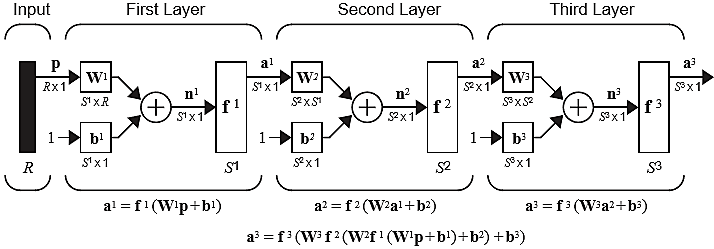
\includegraphics[width=16cm]{img/MLP.png}
        \caption{Perceptron de tres capas. \cite{libro1}}
        \label{fig:MLP}
    \end{center}
\end{figure}

En donde $S^1$ indica el número de neuronas de la capa uno, $S^2$ el número de neuronas en la capa dos y así consecutivamente. Esta misma estructura permite identificar la arquitectura de la red neuronal donde $R$ es el número de entradas. Para identificar el conjunto de funciones que se utiliza en cada capa se utiliza.

\[ \begin{bmatrix} F^1 & F^2 & F^3 & \dots & F^N \end{bmatrix} \]


Cada uno de estos elementos hace referencia alguna función de activación, las funciones que más se suelen utilizar son no lineales algunas de estas son.

\begin{itemize}
    \item Log-Sigmoid
    \[ a = \dfrac{1}{1+e^{-n}}\]
    \item Hyperbolic Tangent Sigmoid
    \[ a = \dfrac{e^n - e^{-n}}{e^n + e^{-n}}\]
    \item Linear
    \[ a = n\]
\end{itemize}

\begin{figure}[H]
    \begin{center}
        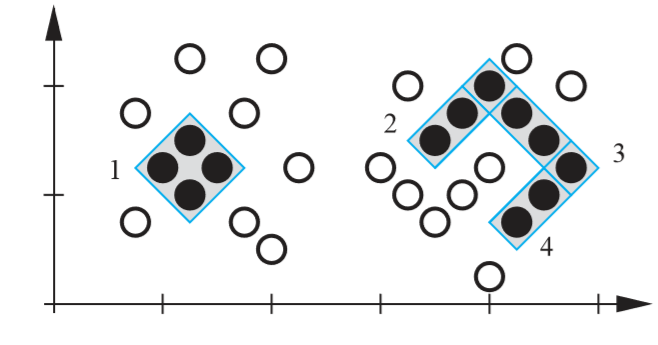
\includegraphics[width=7cm]{img/patrones.png}
        \caption{Clasificación de patrones. \cite{libro1}}
        \label{fig:clasificacion}
    \end{center}
\end{figure}

Las principales aplicaciones del MLP son:
\begin{itemize}
    \item Clasificación de patrones, objetos y caracteres como en la figura \ref{fig:clasificacion}.
    \item Aproximación de funciones.
    \item Compresión y codificación de información
    \item Reconocimiento de palabras (véase figura \ref{fig:palabras}).
    \item Segmentación de imágenes \cite{pdf}.
\end{itemize}

\begin{figure}[H]
    \begin{center}
        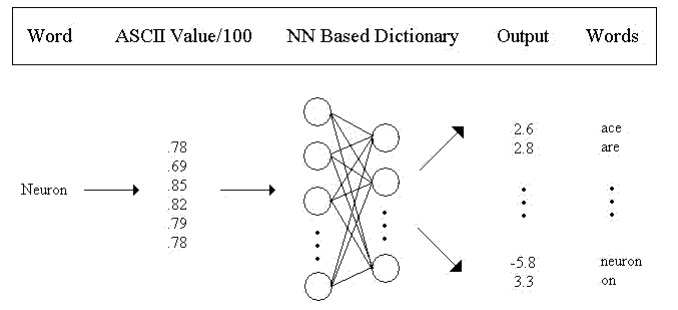
\includegraphics[width=12cm]{img/palabras.png}
        \caption{Diagrama del reconocimiento de palabras. \cite{pdf}}
        \label{fig:palabras}
    \end{center}
\end{figure}

La aproximación de señales se usa en sistemas de control en donde se trata de encontrar una función que pueda mapear mediciones de salidas a controles de entrada. Se puede realizar la aproximación de cualquier función si se tienen suficientes neuronas en las capas ocultas. 
\subsection{Backpropagation}
Para el estudio de backpropagation es importante conocer las ecuaciones que se usan en el aprendizaje que realiza. La primera de ellas está relacionada con las salidas de cada capa del MLP, estas ecuaciones son otra forma de representar la arquitectura de la figura \ref{fig:MLP}.

\begin{equation} \label{eq:1}
\boldsymbol{a}^0 = \boldsymbol{p}
\end{equation}
\begin{equation} \label{eq:2}
\boldsymbol{a}^{m+1} = \boldsymbol{f}^{m+1}(\boldsymbol{W}^{m+1}\boldsymbol{a}^{m}+\boldsymbol{b}^{m+1}
), \quad \text{Para $m=0, 1, \ldots M-1$}
\end{equation}
\begin{equation} \label{eq:3}
    \boldsymbol{a} = \boldsymbol{a}^{M}
\end{equation}
El valor de $M$ es el número de capas que tiene la red. La ecuación \ref{eq:1} hace referencia a que la capa uno tiene como entrada el conjunto de datos $\boldsymbol{p}$. Por otro lado la ecuación \ref{eq:3} es considerado como la salida final de la red neuronal.

El algoritmo backpropagation es una generalización del algoritmo LMS ya que ambos utilizan el error cuadrático medio, además utiliza un conjunto de entrenamiento compuesto por la entrada a la red y su correspondiente salida objetivo.
\[ \left\lbrace \boldsymbol{p_1}, \boldsymbol{t_1} \right\rbrace, \left\lbrace \boldsymbol{p_2}, \boldsymbol{t_2} \right\rbrace, \dots, \left\lbrace \boldsymbol{p_Q}, \boldsymbol{t_Q} \right\rbrace  \]

\subsection{ECUACIONES QUE PODRÍA ESTAR OCUPANDO}
\subsubsection{Forward propagation}
\begin{align*}
 \boldsymbol{a}^0 &= \boldsymbol{p} \\
 \boldsymbol{a}^{m+1} = 
\boldsymbol{f}^{m+1}(\boldsymbol{W}^{m+1}\boldsymbol{a}^{a}+\boldsymbol{b}^{m+1}
) & & \text{Para $m=0, 1, \ldots M-1$} \\
 \boldsymbol{a} &= \boldsymbol{a}^{M}
\end{align*}
\subsubsection{Backward propagation}
\begin{align*}
    \boldsymbol{s}^M &= 
-2\boldsymbol{\dot{F}}^{M}(\boldsymbol{n}^{M})(\boldsymbol{t-a}) \\
    \boldsymbol{s}^{m} &= 
\boldsymbol{\dot{F}}^{m}(\boldsymbol{n}^{m})(\boldsymbol{W}^{m+1})^{T}
\boldsymbol{s}^{m+1} & & \text{para $m=M-1, \ldots, 2, 1$} \\
\text{donde} \\
\boldsymbol{\dot{F}}^{m}(\boldsymbol{n}^{m}) &=
\begin{bmatrix}
  \dot{f}^{m}(n_{1}^{m}) & 0 & \ldots & 0 \\
  0 & \dot{f}^{m}(n_{2}^{m}) & \ldots & 0 \\
  \vdots & \vdots & \ddots & \vdots \\
  0 & 0 & \ldots & \dot{f}^{m}(n_{s^{m}}^{m})
\end{bmatrix} \\
\dot{f}^{m}(n_{j}^{m}) &= 
\frac{\partial \dot{f}^{m}(n_{j}^{m})}{\partial n_{j}^{m}}
\end{align*}
\subsubsection{Actualización de los pesos}
\begin{align*}
    \boldsymbol{W}^{m}(k+1) &= W^{m}(k)-\alpha 
\boldsymbol{s}^{m}(\boldsymbol{a}^{m-1})^{T}, \\
\boldsymbol{b}^{m}(k+1) &= \boldsymbol{b}^{m}(k) - \alpha \boldsymbol{s}^{m}
\end{align*}

\newpage

\section{Resultados experimentales}
Se realizaron 3 experimentos para comprobar el funcionamiento del perceptrón multicapa, para cada experimento se introdujeron valores diferentes para cada parámetro de la arquitectura, esto debido a que cada función a aproximar necesita parámetros personalizados para su correcto funcionamiento.

Algunas constantes que se mantienen en todos los experimentos son que la entrada de datos y objetivos se realizan mediante archivos de texto, además para cada experimento se muestra la evolución del error de iteración de entrenamiento y de validación en estas gráficas se puede observar que el error de validación tiende a ser más alto que el error de entrenamiento.

También, se gráfica la evolución de pesos y bias para cada capa de la red neuronal, finalmente se muestra una comparación entre un conjunto de prueba y la salida que proporciona el MLP. Además de imprimir los valores finales de error de iteración, error de validación y error de prueba. Finalmente los valores finales de pesos y bias son almacenados en un archivo de texto, uno por cada capa de la red.
\subsection{Experimento 1}
Se trabajo con un conjunto de datos con 101 datos los cuales al graficar dan como resultado la figura \ref{fig:original1}.

Los valores que se ingresaron son los que se muestran en la figura \ref{fig:entrada1} los valores más importantes que se tienen aquí son el factor de aprendizaje $\alpha=0.03$ el máximo numero de iteraciones a realizar el cual fue $iteraciones_{max} = 5000$ junto a un error permitido de $E_{it} = 0.005$ mientras que cada $200$ iteraciones se hará una iteración de validación con un máximo de tres incrementos consecutivos.
\begin{figure}[H]
    \begin{center}
        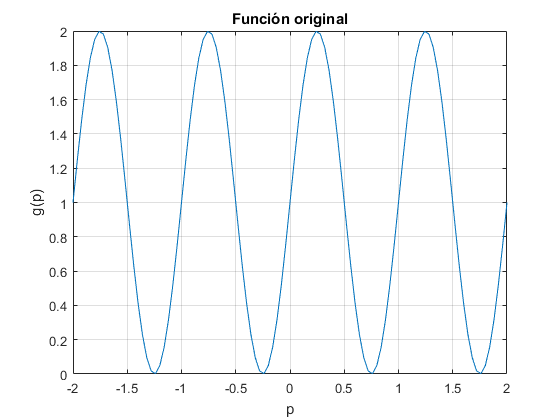
\includegraphics[width=10cm]{1/original.png}
        \caption{Función a aproximar en el experimento 1.}
        \label{fig:original1}
    \end{center}
\end{figure}
Para realizar las iteraciones de entrenamiento, prueba y validación la división del conjunto de datos fue $80-10-10$ respectivamente. Por otro lado, la arquitectura fue la siguiente.
\[ \left[ 1 \quad 6 \quad 1 \right] \]
\[ \left[ 3 \quad 1 \right] \]
donde
\begin{itemize}
    \item $3$ hace referencia a la función $tansig$.
    \item $1$ es la función $purelin$.
\end{itemize}
Una representación gráfica de esta arquitectura es la que se muestra en la figura \ref{fig:arqui1}. Los valores de pesos y bias de cada capa son inicializados entre $-1$ y $1$.
\begin{figure}[H]
    \begin{center}
        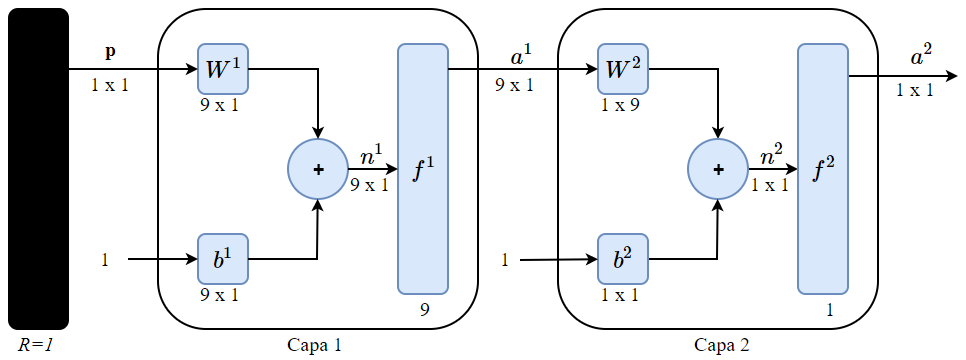
\includegraphics[width=14cm]{img/arqui1.png}
        \caption{Arquitectura del primer experimento.}
        \label{fig:arqui1}
    \end{center}
\end{figure}
Como se puede observar la primera capa tiene seis neuronas mientras que la segunda sólo tiene 1.
\begin{figure}[H]
    \begin{center}
        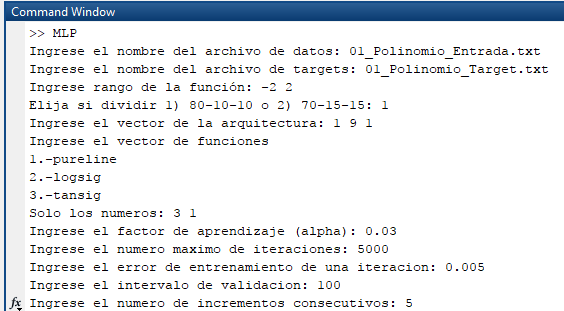
\includegraphics[width=14cm]{1/entrada.png}
        \caption{Entrada de datos del experimento 1.}
        \label{fig:entrada1}
    \end{center}
\end{figure}
Los errores finales se pueden observar en la figura \ref{fig:salida1}, además de que la condición de finalización fue que se alcanzo el número máximo de iteraciones.
\begin{figure}[H]
    \begin{center}
        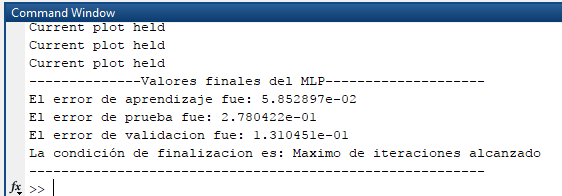
\includegraphics[width=14cm]{1/salida.png}
        \caption{Errores de cada iteración del experimento 1.}
        \label{fig:salida1}
    \end{center}
\end{figure}
Las siguientes imágenes son la evolución de pesos y bias de cada capa. Cada gráfica tiene comportamientos diferentes pero algo en lo que se parecen es que en algún punto de la gráfica ya no se producen tantas modificaciones en los valores que presentan.
\begin{figure}[H]
    \begin{center}
        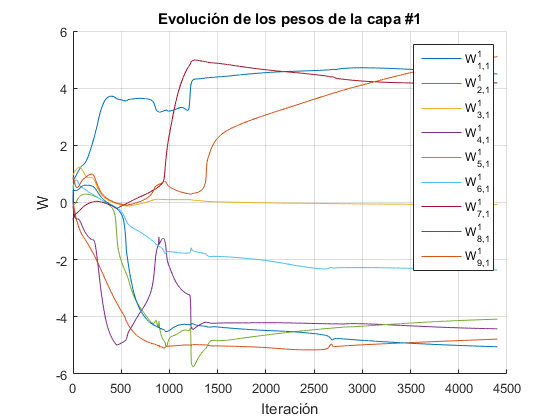
\includegraphics[width=12cm]{1/pesos1.png}
        \caption{Evolución de los pesos de la capa 1 del experimento 1.}
        \label{fig:pesos1}
    \end{center}
\end{figure}

\begin{figure}[H]
    \begin{center}
        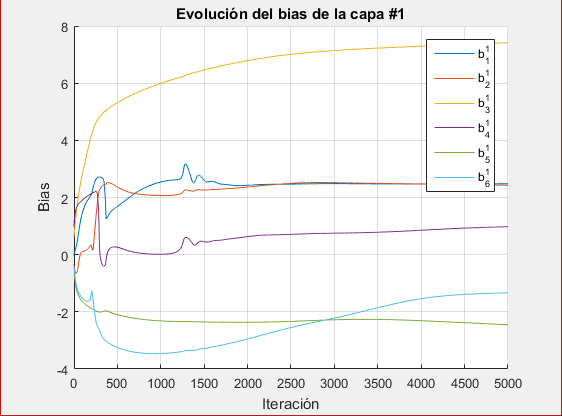
\includegraphics[width=12cm]{1/bias1.png}
        \caption{Evolución de los bias de la capa 1 del experimento 1.}
        \label{fig:bias1}
    \end{center}
\end{figure}

\begin{figure}[H]
    \begin{center}
        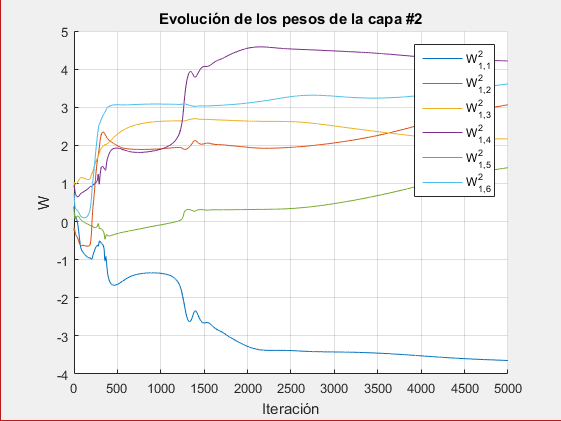
\includegraphics[width=12cm]{1/pesos2.png}
        \caption{Evolución de los pesos de la capa 2.}
        \label{fig:pesos2}
    \end{center}
\end{figure}

\begin{figure}[H]
    \begin{center}
        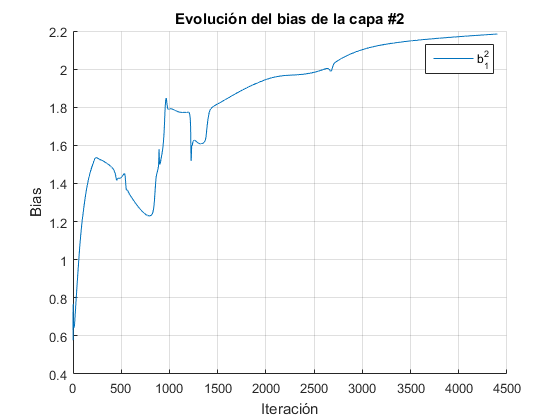
\includegraphics[width=12cm]{1/bias2.png}
        \caption{Evolución de los bias de la capa 2.}
        \label{fig:bias2}
    \end{center}
\end{figure}
Debido a que la división de los datos de entrada fue $80-10-10$ sólo se tienen $10$ datos que propagar se producen demasiados picos, por otro lado la aproximación se realiza casi completamente.
\begin{figure}[H]
    \begin{center}
        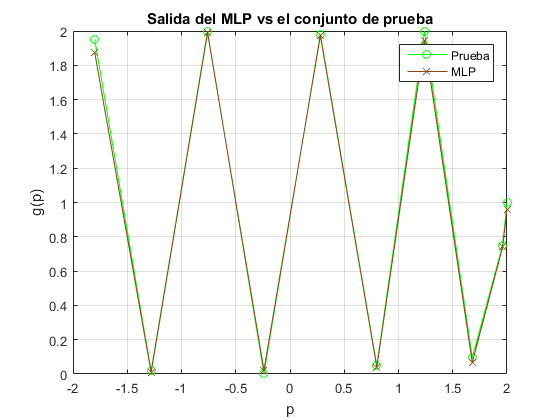
\includegraphics[width=12cm]{1/prueba.png}
        \caption{Comparación de las gráficas}
        \label{fig:prueba1}
    \end{center}
\end{figure}
Se puede observar que el error llega un punto en el que disminuye de una manera muy lenta hasta el final de todas las iteraciones.
\begin{figure}[H]
    \begin{center}
        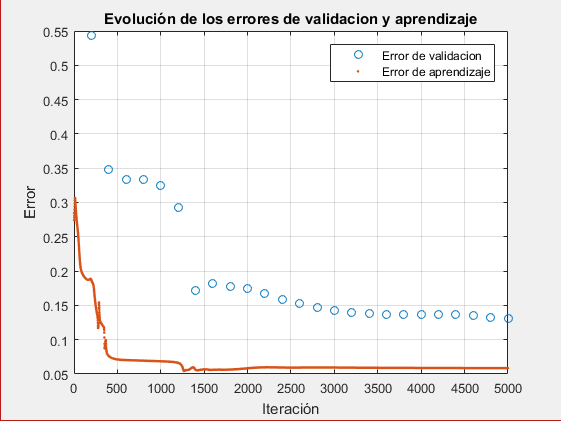
\includegraphics[width=12cm]{1/error.png}
        \caption{Evolución de los errores del experimento 1.}
        \label{fig:error1}
    \end{center}
\end{figure}
\newpage

\subsection{Experimento 2}
Para este experimento se trato con 241 datos los cuales al graficar dan como resultado la figura \ref{fig:original2}.

Los valores que se ingresaron son los que se muestran en la figura \ref{fig:entrada2} los valores más importantes que se tienen aquí son el factor de aprendizaje $\alpha=0.01$ el máximo numero de iteraciones a realizar el cual fue $iteraciones_{max} = 5000$ junto a un error permitido de $E_{it} = 0.0005$ mientras que cada $100$ iteraciones se hará una iteración de validación con un máximo de tres incrementos consecutivos.
\begin{figure}[H]
    \begin{center}
        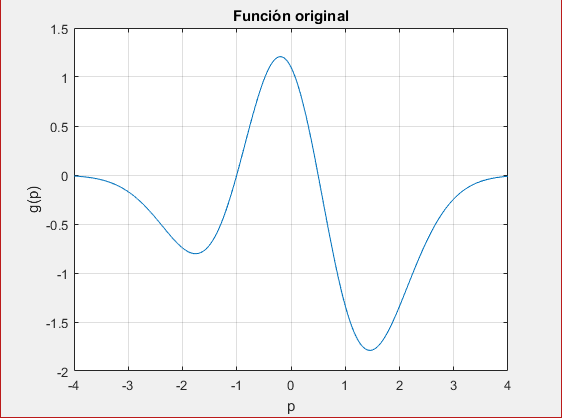
\includegraphics[width=10cm]{2/original.png}
        \caption{Función a aproximar en el experimento 2.}
        \label{fig:original2}
    \end{center}
\end{figure}
En esta ocasión la división de los datos fue $70-15-15$ para conjunto de entrenamiento, prueba y validación respectivamente. Por otro lado, la arquitectura fue la siguiente.
\[ \left[ 1 \quad 6 \quad 1 \right] \]
\[ \left[ 2 \quad 1 \right] \]
donde
\begin{itemize}
    \item $3$ hace referencia a la función $logsig$.
    \item $1$ es la función $purelin$.
\end{itemize}
Una representación gráfica de esta arquitectura es la que se muestra en la figura \ref{fig:arqui2}. Los valores de pesos y bias de cada capa son inicializados entre $-1$ y $1$.
\begin{figure}[H]
    \begin{center}
        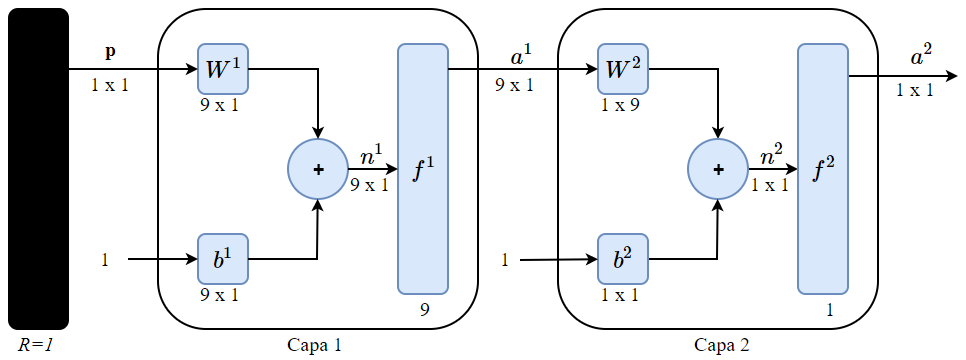
\includegraphics[width=14cm]{img/arqui1.png}
        \caption{Arquitectura del segundo experimento.}
        \label{fig:arqui2}
    \end{center}
\end{figure}
De nueva cuenta se tienen seis neuronas en la primera capa y sólo una en la segunda.
\begin{figure}[H]
    \begin{center}
        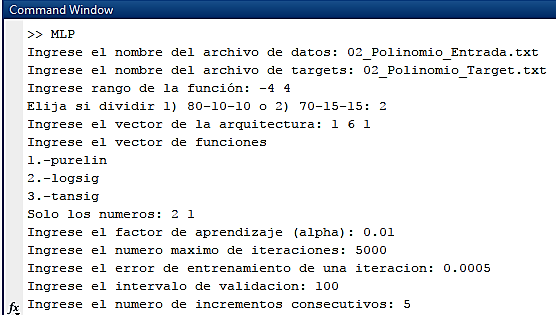
\includegraphics[width=14cm]{2/entrada.png}
        \caption{Entrada de datos del experimento 2.}
        \label{fig:entrada2}
    \end{center}
\end{figure}
Los errores finales fueron, para el error de validación fue $2.61 x 10^{-3}$, para el de prueba fue $2.37x10^{-3}$ mientras que para el de aprendizaje fue $4.49x10^{-4}$ dichos valores se encuentran en la figura \ref{fig:salida2}, además de que la condición de finalización fue que el error de aprendizaje fue menor que el error de iteración.
\begin{figure}[H]
    \begin{center}
        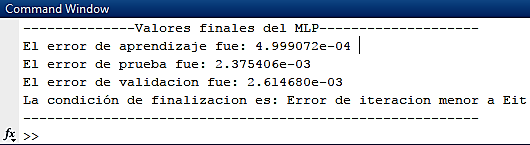
\includegraphics[width=14cm]{2/salida.png}
        \caption{Errores de cada iteración del experimento 2.}
        \label{fig:salida2}
    \end{center}
\end{figure}
Las siguientes imágenes son la evolución de pesos y bias de cada capa. Cada gráfica tiene comportamientos diferentes pero algo en lo que se parecen es que en algún punto de la gráfica ya no se producen tantas modificaciones en los valores que presentan.
\begin{figure}[H]
    \begin{center}
        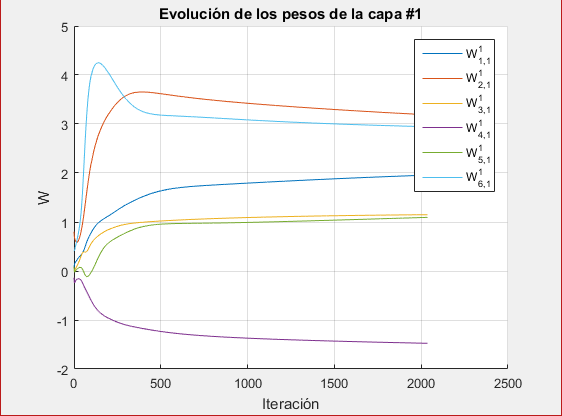
\includegraphics[width=12cm]{2/pesos1.png}
        \caption{Evolución de los pesos de la capa 1 del experimento 2.}
        \label{fig:pesos3}
    \end{center}
\end{figure}

\begin{figure}[H]
    \begin{center}
        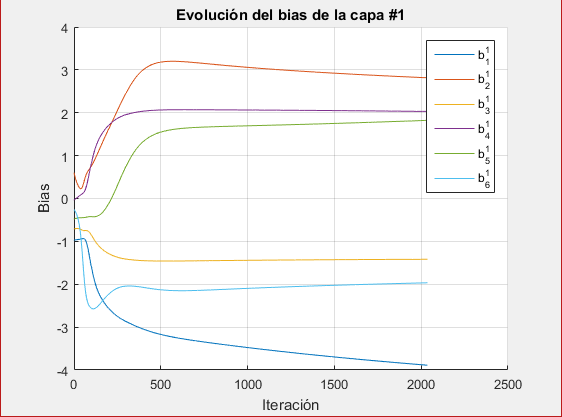
\includegraphics[width=12cm]{2/bias1.png}
        \caption{Evolución de los bias de la capa 1 del experimento 2.}
        \label{fig:bias3}
    \end{center}
\end{figure}

\begin{figure}[H]
    \begin{center}
        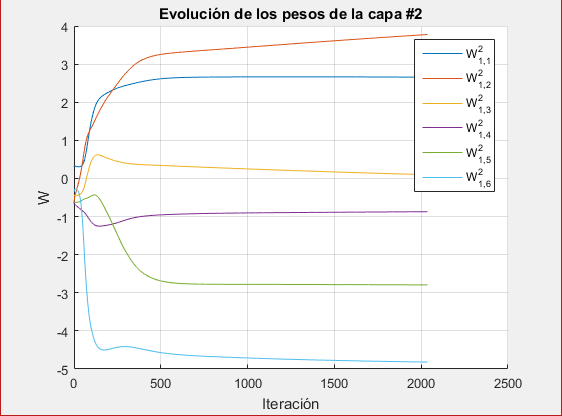
\includegraphics[width=12cm]{2/pesos2.png}
        \caption{Evolución de los pesos de la capa 2.}
        \label{fig:pesos4}
    \end{center}
\end{figure}

\begin{figure}[H]
    \begin{center}
        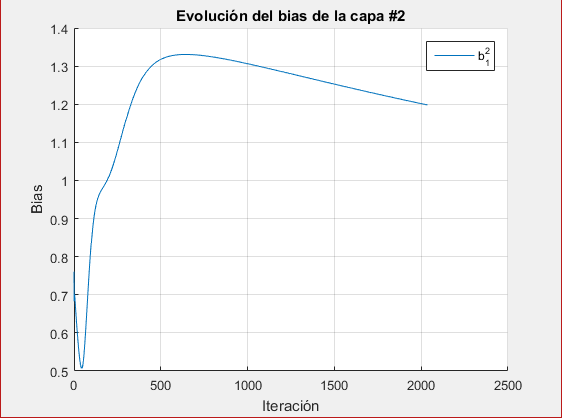
\includegraphics[width=10cm]{2/bias2.png}
        \caption{Evolución de los bias de la capa 2.}
        \label{fig:bias4}
    \end{center}
\end{figure}
Finalmente tenemos la comparación de la salida del MLP y los valores reales, ya que el error es muy bajo la aproximación se realiza en casi todos los puntos con excepción de los primeros valores de la gráfica
\begin{figure}[H]
    \begin{center}
        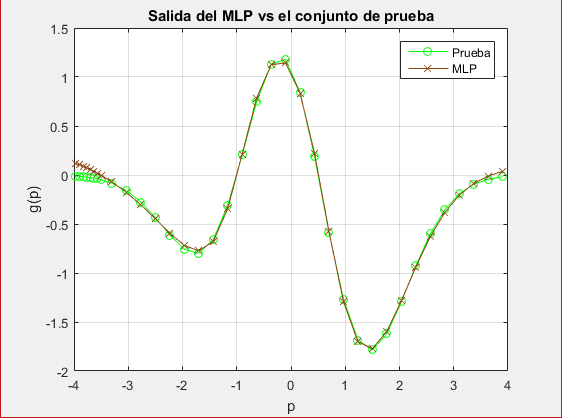
\includegraphics[width=12cm]{2/prueba.png}
        \caption{Comparación de las gráficas}
        \label{fig:prueba2}
    \end{center}
\end{figure}
El comportamiento de los errores se puede ver reflejado en la evolución del error en el cual incluso el error de validación es más pequeño con cada iteración que se genera.
\begin{figure}[H]
    \begin{center}
        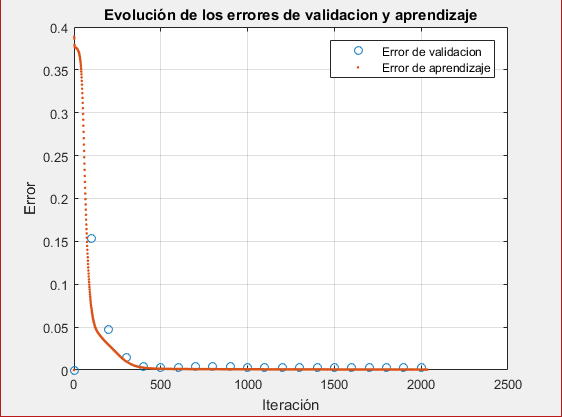
\includegraphics[width=14cm]{2/error.png}
        \caption{Evolución de los dos errores.}
        \label{fig:error2}
    \end{center}
\end{figure}

\newpage

\subsection{Experimento 3}

\section{Discusión de resultados}
\section{Conclusiones}
\bibliographystyle{apalike}
\bibliography{reporte}
\section{Anexo}

\end{document}
